\chapter{Improve the Base Model}



The base model in previous chapter does not show the results as we expected. In this chapter we look into that problem, and figure out three aspects to improve over the base model.


\section{Use a count prediction model}



\subsection{Linear regression gives negative prediction}

One obvious drawback is that the linear regression is not a count prediction model, since it will give negative number as prediction. For example, we find the suspicious community \#32 case. Refer to Figure~\ref{fig:crime-ca}, we know this community is the downtown. The crime count for community \#32 is $7,709$ in 2010. However, the linear regression base model gives $-1,448$ as prediction. This result is not acceptable in a count prediction model. We further look into the features of community \#32 to figure out why it has negative crime count estimation. It turns out that community \#32 has $12,175$ venues in total, which is 10 times more than the average of other communities ($1,011$). In our learned model, the venue count feature has a negative coefficients, which indicates that popular places tend to have less crime incidents. The big difference in the venue count feature lead to a negative prediction for community \# 32.




\subsection{Poisson regression as a count prediction model}

To address this issue, a count prediction model is a natural selection. The \emph{Poisson regression} is another form of regression, more appropriate for count data than linear regression \cite{GMS95}\cite{Lamb92}. With shortened notation $X$, Poisson regression model has the exponential function as link function
\begin{equation}
\label{eq:prm}
E(y) = e^{X w}.
\end{equation}
This comes from the assumption that $y$ follows Poisson distribution with mean $\lambda $. Additionally, the mean $lambda$ is determined by observed independent variables $X$, with the link function $\lambda = e^{Xw}$. Adding all together, the joint probability of $y$ is 
\begin{equation}
P(y|w) = \frac{e^{-e^{Xw}}(e^{Xw})^y}{y!}.
\end{equation}


Compared with the linear regression, the negative log-likelihood function of Poisson regression is derived from the dependent variable itself, unlike linear regression, which is derived from the joint distribution of error term. 


However, Poisson regression enforces the mean and variance of dependent variable $y$ to be equal. This restriction leads to the ``over-dispersion'' issue for some real problems, that is the presence of larger variability in data set than the statistical model expected. In our crime dataset, the mean of crime count for all communities is $4,787$, while the variance is $1.6 \times 10^7$. The variance is almost the square of the mean, which significantly violate the Poisson distribution assumption. Therefore, we should look for other count prediction model.





\subsection{Negative binomial regression addresses over-dispersion}

To allow larger variance in the predicted value,  we introduce the Poisson-Gamma mixture model, which is also known as \emph{negative binomial regression}.  The negative binomial regression has been used in similar work~\cite{Osg00}.




Given that the crime rate $y$ follows Poisson distribution with mean $\lambda$.  In order to allow for larger variance, now the $\lambda$ itself is a random variable, distributed as a Gamma distribution with shape $k=r$ and scale $\theta = \frac{1-p}{p}$.  The probability function of $y$ becomes
\begin{align}
P(y| r, p) & = \int_0^{\infty} P_{Poisson}(y|\lambda) \cdot P_{Gamma}(\lambda|r, p) d \lambda \nonumber \\ 
		& = \int_0^{\infty} \frac{\lambda^y}{y!} e^{-\lambda} \cdot \lambda^{r-1} \frac{e^{-\lambda(1-p)/p}}{(\frac{p}{1-p})^y \Gamma(r)} d\lambda  \nonumber \\
		& = \frac{\Gamma(r+y)}{y! \Gamma(r)} p^k (1-p)^y
\end{align}
This is exactly the probability density function of negative binomial distribution.


In negative binomial regression, the link function is
\begin{equation}
E(y) = e^{X w + \epsilon}.
\end{equation}
The error term $e^\epsilon$ is the mixture prior, and we assume it follows Gamma distribution with shape parameter $k=\frac{1}{\theta}$, so that it has mean $E(e^\epsilon) = k\theta = 1$ and variance $Var(e^\epsilon) = k\theta^2 = \theta$. This setting ensures the $E(y) = e^{Xw} \cdot e^\epsilon = e^{Xw}$.



\subsection{Evaluation of negative binomial regression model}



\subsubsection{Evaluation Settings}

We adopt the leave-one-out evaluation to estimate the crime rate of one geographic region given all the information of all the other regions. When we construct the spatial/social lag variable for the training data, the effect of testing region is completely removed. For example, if region $y_t$ is the testing region, the remaining $\{y_i\} \backslash y_t$ become the training set. For any $y_j$ in the training set, its geographical influence feature and taxi flow feature are constructed from $\{y_i\} \backslash \{y_t, y_j\}$.


In the evaluation, we estimate the crime rate for testing community area. The accuracy of estimation is evaluated by mean absolute error (MAE) and mean relative error (MRE).

\begin{align}
MAE & = \frac{\sum_i^n |y_i - \hat{y_i}| }{n} \\
MRE & = \frac{\sum_i^n |y_i - \hat{y_i}|} {\sum_i^n y_i }
\end{align}


\subsubsection{Performance Study: Negative Binomial Regression vs. Linear Regression}


We evaluate the estimation accuracy under various feature combinations. The leave-one-out evaluation results are shown in Table~\ref{tb:perf}.  We run both linear regression model and negative binomial model on five consecutive years, 2010 -- 2014. Both MAE and MRE are shown in the table. We have four types of features, demographics, POI, geographical influence and taxi flow. We test the various settings of feature combinations.





\begin{table}[htb]
\centering
\caption{Performance evaluation. Various feature combinations are shown in each column. The linear regression model and negative binomial results are compared by year group. }
\vspace{2mm}
\label{tb:perf}
\begin{tabular}{|c|c|c|c|c|c|c|c|c|c|c|}
\hline
\multicolumn{3}{|c|}{} & \multicolumn{8}{|c|}{Settings} \\ \hline
\multicolumn{3}{|c|}{Column ID} & 1 & 2 & 3 & 4 & 5 & 6 & 7 & 8 \\ \hline
\multicolumn{2}{|c|}{\multirow{4}{*}{Features$^1$}}	& D & \checkmark & \checkmark&\checkmark & \checkmark & \checkmark& \checkmark& \checkmark& \checkmark \\ \cline{3-11}
\multicolumn{2}{|c|}{}	& G & & & & & \checkmark & \checkmark& \checkmark& \checkmark \\ \cline{3-11}
\multicolumn{2}{|c|}{}	& P & & \checkmark & & \checkmark & &\checkmark & & \checkmark \\ \cline{3-11}
\multicolumn{2}{|c|}{}	& T & & & \checkmark& \checkmark & & & \checkmark& \checkmark \\ \hline
Year & Model$^2$ & Error & \multicolumn{8}{|c|}{} \\ \hline
	\cellcolor{white}&  \cellcolor{white} & MAE & 394.41 & 416.98 & 408.09 &  406.93  &394.78 &432.45 & 402.25& 416.41\\ \cline{3-11}
	&	\multirow{-2}{*}{LR}& MRE & 0.294& 0.311 & 0.304 & 0.304 & 0.295 &0.323 & 0.300& 0.310\\ \cline{2-11}
	\rowcolor{Gray}
	\cellcolor{white}	& \cellcolor{white} & MAE & 391.53&   333.14 & 395.64 & 323.47 & 389.55&350.06 & 387.43& \textbf{320.75}\\ \cline{3-11}
	\rowcolor{Gray}
	\cellcolor{white}\multirow{-4}{*}{2010}	&\cellcolor{white}\multirow{-2}{*}{NB}	& MRE & 0.292& 0.249 & 0.295 & 0.241 & 0.290& 0.261& 0.289& \textbf{0.239} \\ \hline
	


	\cellcolor{white}	& \cellcolor{white} & MAE & 380.22&   409.30 & 396.97 &  401.11 & 379.61& 422.94&389.39 & 408.91\\ \cline{3-11}
	&	\multirow{-2}{*}{LR}& MRE &0.295  &  0.318  &  0.309 &  0.312 & 0.295 &0.328 & 0.302 & 0.320   \\ \cline{2-11}
	\rowcolor{Gray}
	\cellcolor{white}& \cellcolor{white} & MAE &381.11 & 332.62 & 388.81  & 328.94 & 378.84& 345.24& 381.33& \textbf{335.97} \\ \cline{3-11}
	\rowcolor{Gray}
	\cellcolor{white}\multirow{-4}{*}{2011}	&	\cellcolor{white}\multirow{-2}{*}{NB}& MRE&0.296 & 0.259 & 0.302  & 0.256 & 0.294 & 0.268  & 0.296  & \textbf{0.253}  \\ \hline
	


	\cellcolor{white}& \cellcolor{white} & MAE &378.91 & 412.95 & 401.54  & 412.20& 376.53 & 423.88 & 399.25 & 419.93\\ \cline{3-11}
	&	\multirow{-2}{*}{LR}& MRE& 0.306 & 0.334 & 0.325 & 0.333&  0.304 & 0.343 & 0.322 & 0.339 \\ \cline{2-11}
	\rowcolor{Gray}
	\cellcolor{white}& \cellcolor{white} & MAE & 386.31 & 337.24 & 389.58  & 331.41 & 384.23 & 352.22 & 381.67 & \textbf{345.49} \\ \cline{3-11}
	\rowcolor{Gray}
	\cellcolor{white}\multirow{-4}{*}{2012}&\cellcolor{white}\multirow{-2}{*}{NB}	& MRE& 0.312 & 0.273 & 0.315  & 0.268 & 0.310 & 0.284 & 0.308 & \textbf{0.279} \\ \hline
	

	\cellcolor{white}& \cellcolor{white} & MAE & 367.89 & 420.81 & 390.75  & 402.75 & 369.24 & 433.48 &388.92 & 412.31\\ \cline{3-11}
	&	\multirow{-2}{*}{LR}& MRE& 0.324 &  0.370 & 0.344  & 0.354  & 0.325 & 0.381 & 0.342& 0.362\\ \cline{2-11}
	\rowcolor{Gray}
	\cellcolor{white}& \cellcolor{white}& MAE & 376.08&  333.92 & 373.08 & 312.63 & 377.57 & 350.33 & 368.49 & \textbf{319.86}\\ \cline{3-11}
	\rowcolor{Gray}
	\cellcolor{white}\multirow{-4}{*}{2013}	&	\cellcolor{white}\multirow{-2}{*}{NB} & MRE& 0.331 &   0.294 & 0.328  & 0.275 & 0.332 & 0.308 & 0.324& \textbf{0.281}\\ \hline

	\cellcolor{white}& \cellcolor{white} & MAE & 331.28 & 375.53 & 349.00  & 350.31 & 329.93& 386.90& 345.79& 361.28\\ \cline{3-11}
	&	\multirow{-2}{*}{LR} & MRE& 0.326 & 0.369 & 0.343  & 0.345 & 0.324& 0.380& 0.340& 0.355\\ \cline{2-11}
	\rowcolor{Gray}
	\cellcolor{white}&\cellcolor{white}  & MAE & 340.73 & 293.52  & 339.17  & 274.45 & 336.09& 308.18& 326.07& \textbf{273.27}\\ \cline{3-11}
	\rowcolor{Gray}
	\cellcolor{white}\multirow{-4}{*}{2014}	&	\cellcolor{white}\multirow{-2}{*}{NB}& MRE& 0.335&  0.289 & 0.334 & 0.270 &  0.331 & 0.303& 0.321 & \textbf{0.269}\\ \hline
\end{tabular}

\footnotesize{$^1$ D -- demographic features, G -- geographical influence, P -- POI features, T -- taxi flow feature.\\}
\footnotesize{$^2$ LR -- Linear Regression, NB -- Negative Binomial Regression.}
\end{table}




We compare the estimation error of negative binomial model with the linear regression base model. We use a incremental settings, where new features are added on top of previous one. The results are shown in Figure~\ref{fig:lrvsnb}.


\begin{figure}[h]
\centering
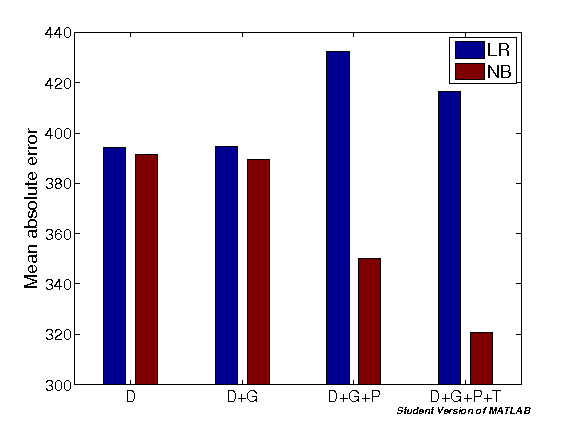
\includegraphics[width=0.8\textwidth]{fig/lrvsnb.png}
\caption{The inference error for linear regression base model. $^*$D -- demographic features, G -- geographical influence, P -- POI features, T -- taxi flow feature}
\label{fig:lrvsnb}
\end{figure}



It is clear that the negative binomial model significantly outperform the linear regression model. Meanwhile, the negative binomial model captures our intuition well. Namely, adding new features will effectively improve the estimation accuracy.


In Table~\ref{tb:perf},  we can see that in different years and under most settings, the negative binomial regression significantly outperforms the linear regression (with only a few exceptions when using only demographic feature). When using all the features, NB is significantly better than LR with at least $6\%$ improvement in relative error.
One reason is that the negative binomial is a count prediction model, which assumes some distribution for the predicted variable and guarantee its positivity. Another reason is that it is difficult to get very precise estimation of crime rate, and  negative binomial model allows a large variance in the estimated crime rate. Therefore negative binomial is more appropriate for crime rate estimation than linear regression.






\section{Capture spatial non-stationarity (Proposed problem 1)}




\subsection{Dynamic spatial model}


We use various types of data to estimate the crime count in community area (CA) of Chicago. For each CA we have observations on crime count and demographics. For each pair of CAs we also have observations on the taxi flow and spatial distance. One straightforward method is to build a regression model from all the features we observed to the crime counts.

We have one interesting observations is that in the south and north part of Chicago, the significance of different features are different. Therefore, the idea is to learn a dynamic weights for different spatial region.



Suppose we have $n$ regions in total, $R = \{ r_1, r_2, \cdots, r_n \}$.
The following notations are used

\begin{table}[h]
\centering
\begin{tabular}{|l|r|}
\hline
crime count at $r_i$ & $y_i$ \\ \hline
demographics at $r_i$ & $\mathbf{d}_i$ \\ \hline
taxi flow between $r_i$ and $r_j$ & $f_{ij}$ \\ \hline
taxi flow weight matrix for $r_i$ & $\mathbf{f_i}$ \\ \hline
spatial weight matrix for $r_i$ & $\mathbf{g_i}$ \\ \hline
social flow lag variable for $r_i$ & $s_i = \mathbf{f}_i^T \mathbf{y}$ \\\hline
spatial flow lag variable for $r_i$ & $p_i = \mathbf{g}_i^T \mathbf{y}$ \\\hline
\end{tabular}
\caption{Symbols for the dynamic coefficient model.}
\end{table}


\subsubsection{Dynamic linear regression model}



For simplicity we use linear regression model
\[
y_i = \mathbf{w}_1^T \mathbf{d}_i + w_2 s_i + w_3 p_i + w_4,
\]
where $\{ w \}$ are the coefficients.

To simplify notations, we use $\mathbf{x}_i$ denote all the available predictors for region $r_i$,
\[
\mathbf{x}_i = [ \mathbf{d}_i, s_i, p_i, 1 ].
\]
Then the model becomes 
\[
y_i = \mathbf{w}^T \mathbf{x}_i.
\]



Now we use a dynamic model, where $\mathbf{w}$ is different for various regions.
This leads to 
\[
y_i  = \mathbf{w}_i^T \mathbf{x}_i.
\]


The problem with formulation is that there are too many parameters to learn. To address this issue, we use the constraint that \textbf{spatially adjacent regions share similar coefficients}.

We use $S_{ij}$ to denote the adjacency of $r_i$ and $r_j$. And the aforementioned constraint is formulated as
\[
\min \sum_{i,j} S_{ij} ||\mathbf{w}_i^T - \mathbf{w}_j^T||_2^2
\] The several choice of $S_{ij}$
\begin{itemize}
\item Binary indicator. $S_{ij} = 1$ if two regions are contiguous, otherwise $S_{ij} = 0$.
\item The reverse distance between $r_i$ and $r_j$. 
\end{itemize}

The overall objective is

\begin{equation}
\label{eq:obj}
\min_{\mathbf{W}}  \sum_i || y_i - \mathbf{w}_i^T \mathbf{x}_i ||_2^2 + \eta \sum_{i,j} S_{ij} ||\mathbf{w}_i^T - \mathbf{w}_j^T||_2^2 
+ \theta || \mathbf{W} ||_F^2
\end{equation}




\subsubsection{Optimization}


Rewrite the Frobenius norm in the last term
\[
|| \mathbf{W} ||_F^2 = \sum_i || \mathbf{w}_i - \mathbf{0}||_2^2.
\]


Therefore the Equation~\ref{eq:obj} is rewritten as
\begin{equation}
\label{eq:obj2}
\min_{\mathbf{W}}  \sum_i || y_i - \mathbf{w}_i^T \mathbf{x}_i ||_2^2 + \eta \sum_{i,j \in 0, \cdots, N} S_{ij} || \mathbf{w}_i - \mathbf{w}_j ||_2^2,
\end{equation}
where $\mathbf{w}_0 = \mathbf{0}$ and $S_{0i} = 1$ for $\forall i$.


To solve the objective in Equation~\ref{eq:obj2}, we use variable splitting. Namely, when optimizing for $\mathbf{w}_i$, we assume all other $\mathbf{w}_{j, j\neq i}$ are fixed. The sub-problem is
\begin{equation}
\label{eq:subobj}
\min_{\mathbf{w}_i}   ||y_i - \mathbf{w}_i^T \mathbf{x}_i ||_2^2 + \eta \sum_j S_{ij}|| \mathbf{w}_i - \mathbf{w}_j||_2^2.
\end{equation}



The update on $\mathbf{w}_i$ is
\[
\mathbf{w}_i = \min_{\mathbf{w}_i}   ||y_i - \mathbf{w}_i^T \mathbf{x}_i ||_2^2 + \eta \sum_j S_{ij} || \mathbf{w}_i - \mathbf{w}_j^{(t)} ||_2^2.
\]

The closed-form solution is

\begin{equation}
\mathbf{w}_i = (\mathbf{x}_i^T \mathbf{x}_i + \eta \sum_j S_{ij} \mathbf{I} )^{-1} (y_i \mathbf{x}_i + \eta \sum_j S_{ij} \mathbf{w}_j) 
\end{equation}


\subsubsection{Inference}

We use the \textbf{leave-one-out} setting to infer and evaluate the crime rate of new community area. 

Suppose the we want to estimate the crime rate $y_i$ of $CA_i$. During the training process, we hold everything about $CA_i$ out (including $y_i$, flow coming in and leaving from $CA_i$). Then training the model on $CA_j$, $\forall j \neq i$, which gives us $w_j$, $\forall j \neq i$. To infer the $y_i$, we need estimate the model coefficient $w_i$ first. Follow the same intuition that model on $CA_i$ is only similar to all its neighboring models, we have
\begin{equation}
\min_{\mathbf{w}_i} \sum_{j, \forall j \neq i} S_{ij} || \mathbf{w}_i - \mathbf{w}_j ||_2^2 + || \mathbf{w}_i ||_2^2
\end{equation}

After getting $\mathbf{w}_i$, we infer $y_i$ by
\begin{equation}
\hat{y}_i = \mathbf{w}_i^T * \mathbf{x}_i
\end{equation}



\section{Consider complicated interaction (Proposed problem 2)}


\subsection{Problem Formulation}

We want to predict the crime rate $y_i$ of each geographical grid (tract/community area) $g_i$. The available observations are demographics features $\x_i$ of each $g_i$ from census, and the interactions among grids. We denote the interactions as $\f_{ij}$ for grid pair $g_i, g_j$, and examples of such interactions are social flow and geospatial distance.

\subsection{Conditional random field model}
The first model comes to mind.

\subsubsection{Potential Function}
Each grid is a node, and its crime rate $y_i$ is the hidden variable that we want to estimate. Two kinds of fixed parameters are observed for each grid $g_i$. The first one is the demographic features $\x_i$. The second is the interactions among grids, such as social flow and geospatial distance, denoted by $\f{ij}$.

We use Conditional Random Field (CRF) shown in Figure~\ref{fig:crf} to model the dependency of nodal features. The learning goal is to estimate the conditional probability of $y$ given $\x$ and $\f$

\begin{equation}
	P(y |  \x, \f) 
\end{equation}


\begin{figure}[hb]
	\centering
	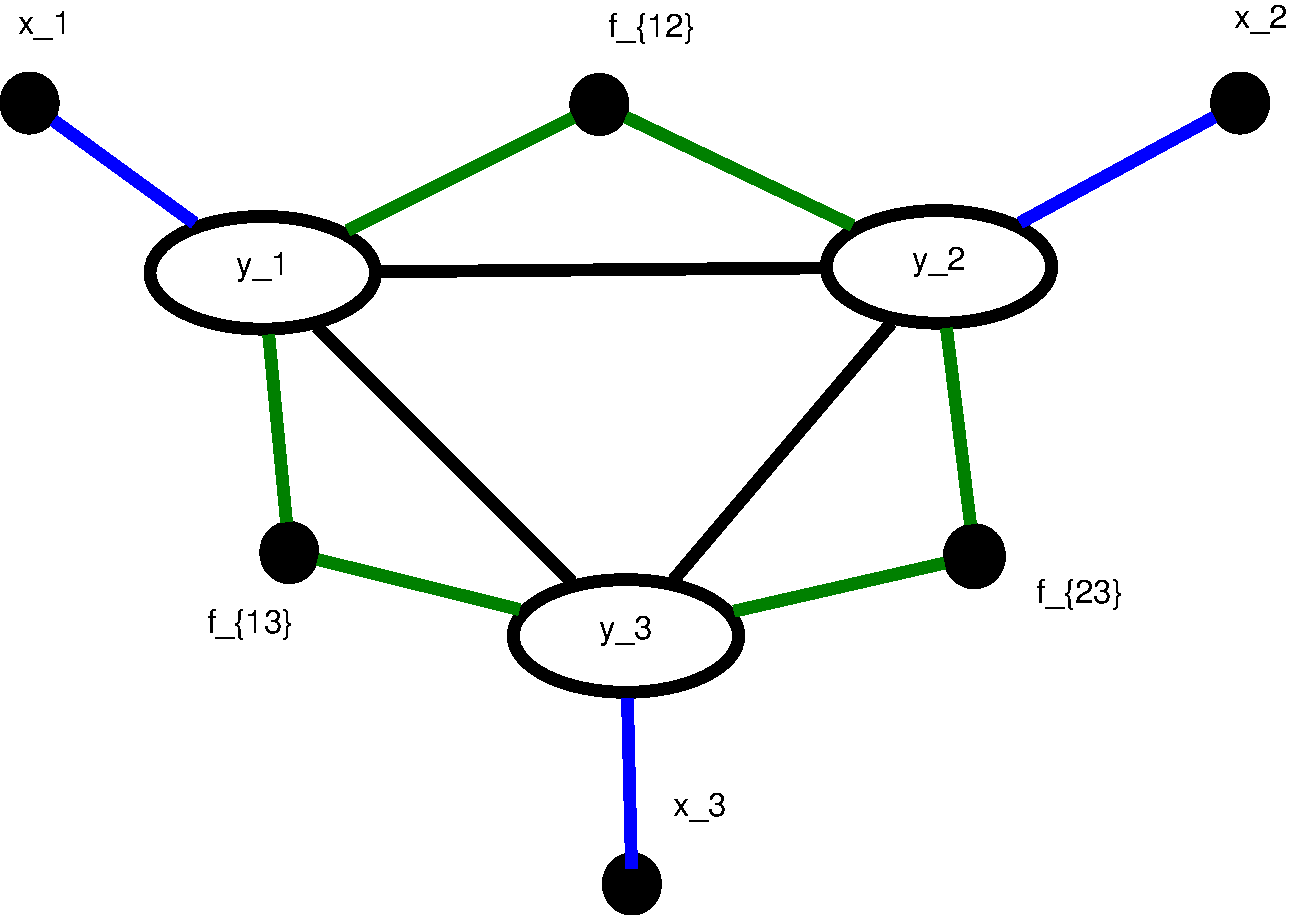
\includegraphics[width=0.5\textwidth]{fig/CRF-fig.pdf}
	\caption{The CRF model of the crime rate $y_i$ for each grid $g_i$.}
	\label{fig:crf}
\end{figure}



In the CRF model, we factorize the probability distribution of $y$ to a series of potential functions $\psi$ on the clique. 
\begin{equation}
	P(Y) = \frac{1}{Z} \prod_{ c \in C} \psi(c)
\end{equation}

Use $C_1$ to denote the set of cliques of size 1 with the form $\langle y_i \rangle$, and $C_2$ to denote size-2 clique. We define the potential function as follows:

\begin{align}
	\psi_{C_1} = &exp( - |y_i - \demow^T \cdot \x_i| )  \forall i \in [1, n], {g_i} \in C_1, \\
	\psi_{C_2} = & exp( - |y_i - y_j - \w^T \cdot \f_{i,j}| )  \forall i,j \in [1, n], {g_i, g_j} \in C_2, 
\end{align}
where $\demow$ and $\w$ are all positive coefficients.

The distribution of $Y$ is given by 
\begin{equation}
	P(Y) =  \frac{1}{Z} \left[ \prod_{i=1}^n \psi_{C_1}(y_i) \times \prod_{i=1}^n \prod_{j=i}^n \psi_{C_2}(y_i, y_j) \right]
\end{equation}
\begin{multline}
	P(Y) =  \frac{1}{Z} exp  \left( - \sum_{i=1}^n |y_i - \demow^T \cdot \x_i| \right. \\
          \left. - \sum_{i=1}^n\sum_{j=i}^n |y_i - y_j - \w^T \cdot \f_{i,j}| \right)
	\label{eq:PY}
\end{multline}


A large value of  potential function $\psi$ implies the high probability of $P(Y)$. The goal is to find a set of $Y$ maximizing $P(Y)$. 


\subsubsection{Inference}


\textbf{Estimate CRF Parameters}
\label{sec:estim}


We solve the Equation~(\ref{eq:PY}) by minimizing the negative log-likelihood function
\begin{multline}
\min_{\demow, \w} -\log P(Y|\demow, \w) = \min_{\demow, \w} \left[ \log Z + \sum_{i=1}^n |y_i - \demow^T \cdot \x_i| \right. \\
\left.  + \sum_{i=1}^n\sum_{j=i}^n |y_i - y_j - \w^T \cdot \f_{i,j}| \right]
\end{multline}

Use matrix form
\[
\min_{\demow, \w} ||X \demow - \y||_1 + ||F \cdot \w - \yp||_1,
\]
where $X$ is demographics matrix with $n$ rows, $\y$ is the $n$-dimension crime rate vector, $F$ is the pairwise features matrix with $(n^2+n)/2$  rows, and $\yp$ is the $(n^2+n)/2$-dimension pairwise crime rate difference vector $\{y_i- y_j\}$.

We can minimize separably.



\textbf{Minimize $\demow$}

\[ \min_{\demow} ||X \demow - \y||_1 \]

Take $X\demow - \y = \z$, and use ADMM.
\begin{multline}
 \min_{\z, \demow}  ||\z||_1 + \rho/2 ||\z - X\demow + \y||_2^2,\\
   s.t.\quad  \z - X\demow + \y = 0 
\end{multline}

\begin{multline}
L(\vec{\theta_1}, \z, \demow) = \max_{\vec\theta_1} \min_{\z, \demow} ||\z||_1 + \\
\rho/2 ||\z - X\demow + \y||_2^2  + \vec{\theta_1}( \z - X\demow + \y ) 
\end{multline}

\textbf{$\demow$ update}

\[ \demow^{k+1} \gets \argmin_{\demow}  \rho/2 ||\z^{k+1} - X\demow + \y + \vec{\theta_1}^{k+1}||_2^2 \]
Take derivative we have
\[ \frac{\partial}{\partial \demow} = \rho X^T(X\demow - \z^{k+1} - \y - \vec\theta_1^{k+1} ) \]
Make it $0$, $\demow^{k+1} = (X^TX)^{-1} X^T(\z^{k+1} + \y + \vec\theta_1^{k+1})$.

\textbf{$\z$ update}

\[ \z^{k+1} \gets \argmin_{\z}  ||\z||_1 + \rho/2 ||\z - X\demow^{k+1} + \y + \vec{\theta_1}^{k+1}||_2^2 \]
So, $\z^{k+1} = S_{1/\rho}(X\demow^{k+1} - \y - \vec\theta_1^{k+1})$.

\textbf{$\vec\theta_1$ update}

\[ \vec\theta_1^{k+1} = \vec\theta_1^{k} + \z^{k+1} - X\demow^{k+1} + \y \]



\textbf{Minimize $\w$}

\[ \min_{\w} ||F \cdot \w - \yp||_1 \]
It has exactly the same form as previously. Therefore,
\begin{multline}
L(\vec{\theta_2}, \z', \w) = \max_{\vec\theta_2} \min_{\z', \w}  ||\z'||_1 + \\
\rho/2 ||\z' - F\w + \yp||_2^2 + \vec{\theta_2}( \z' - F\w + \yp ) 
\end{multline}

\textbf{$\w$ update}
\[ \w^{k+1} = (F^TF)^{-1} F^T(\z^{'k+1} + \yp + \vec\theta_2^{k+1}) \]

\textbf{$\z'$ update}
\[ \z^{'k+1} = S_{1/\rho}(F\w^{k+1} - \yp - \vec\theta_2^{k+1}) \]

\textbf{$\vec\theta_1$ update}
\[ \vec\theta_2^{k+1} = \vec\theta_2^{k} + \z^{'k+1} - F\w^{k+1} + \yp \]



\textbf{Infer New $y_i$}

To infer new $y_i$, we want to maximize the following probability
\[ P(y_i | \x_i, F, \y, \demow, \w), \]
where $\demow$ and $\w$ are estimated using previous section, $\y$ denote the crime rates of other observed geographical units, and $F$ is the pairwise feature matrix.

Take negative log of the probability, we have 

\begin{align}
\min_{y_i} &  \left[ \log Z +  |y_i - \demow^T \cdot \x_i| + \sum_{j \neq i}^n |y_i - y_j - \w^T \cdot \f_{i,j}| \right] \nonumber \\
\min_{y_i} & \left[ |y_i - \demow^T \cdot \x_i| + \sum_{j \neq i}^n |y_i - y_j - \w^T \cdot \f_{i,j}| \right] 
\label{eq:inference}
\end{align}

In Equation~\ref{eq:inference}, we have $n+1$ $\ell_1$-norm terms, which have exactly the same form $|y_i - b_j|$. The objective becomes
\begin{equation}
  \min_{y_i} \sum_j^n |y_i - b_j|,
\label{eq:infy}
\end{equation}
where $b_1 = \demow^T \cdot \x_i$ and $b_j = y_{j-1} + \w^T\cdot \f_{i,j-1}$ for $j > 1$.

Notice that the optimal solution must take value on $\{b_j\}$. We solve this by sorting all the $b_j$ and then calculate the result segment by segment.




